% ======================================================================
\section{Visión general}
El presente documento constituye el modelo de comportamiento del sistema.

Inicialmente se presentan los diagramas de secuencias que modelan 
los eventos que el sistema puede recibir del usuario y los valores de retorno
que produce como consecuencia de estos.

A partir de los diagramas de secuencia del sistema se obtienen las operaciones 
que este presenta. Luego se describen los contratos de cada una de las operaciones.  
% ======================================================================
\section{Diagramas de secuencia del sistema}
\subsection{Interpretar entrada estándar}
\begin{center}
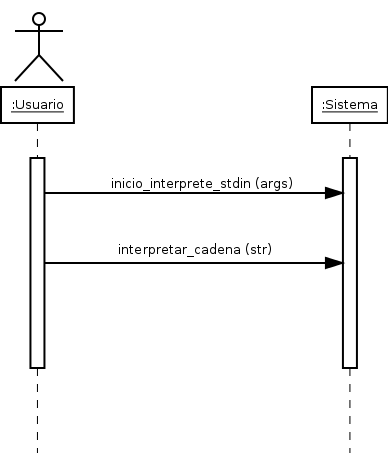
\includegraphics[scale=0.4]{interpretar_stdin.png} \\
\end{center}

\subsection{Interpretar línea}
\begin{center}
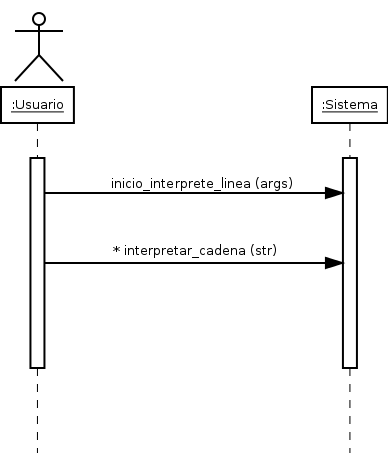
\includegraphics[scale=0.4]{interpretar_line.png} \\
\end{center}

\subsection{Interpretar fichero}
\begin{center}
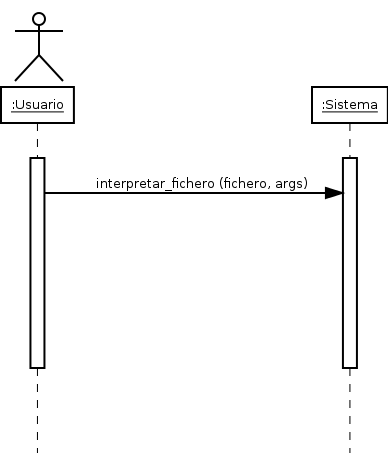
\includegraphics[scale=0.4]{interpretar_file.png} \\
\end{center}

\subsection{Ver ayuda}
\begin{center}
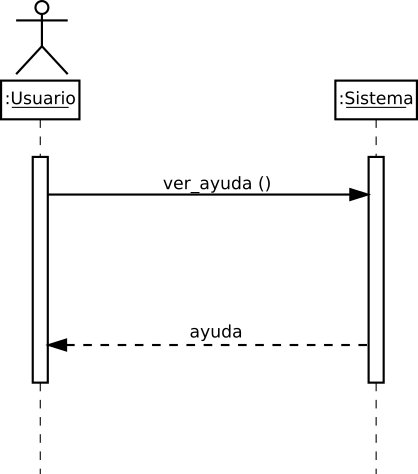
\includegraphics[scale=0.4]{ver_ayuda.png} \\
\end{center}

\subsection{Cargar extensión}
\begin{center}
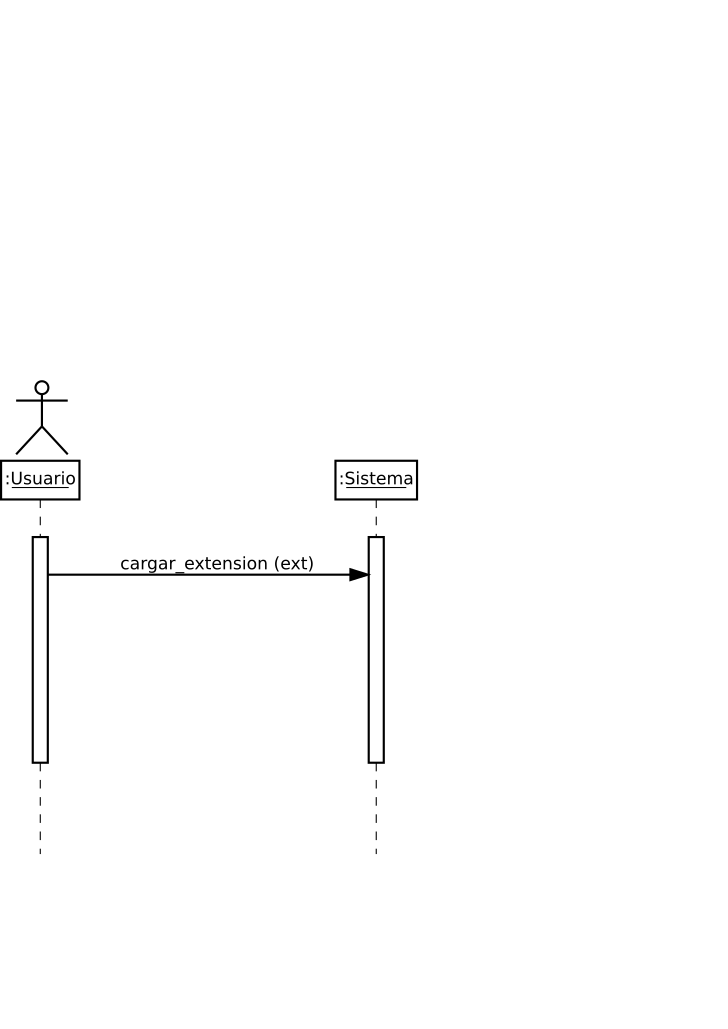
\includegraphics[scale=0.4]{cagar_extension.png} \\
\end{center}

\subsection{Listar extensiones}
\begin{center}
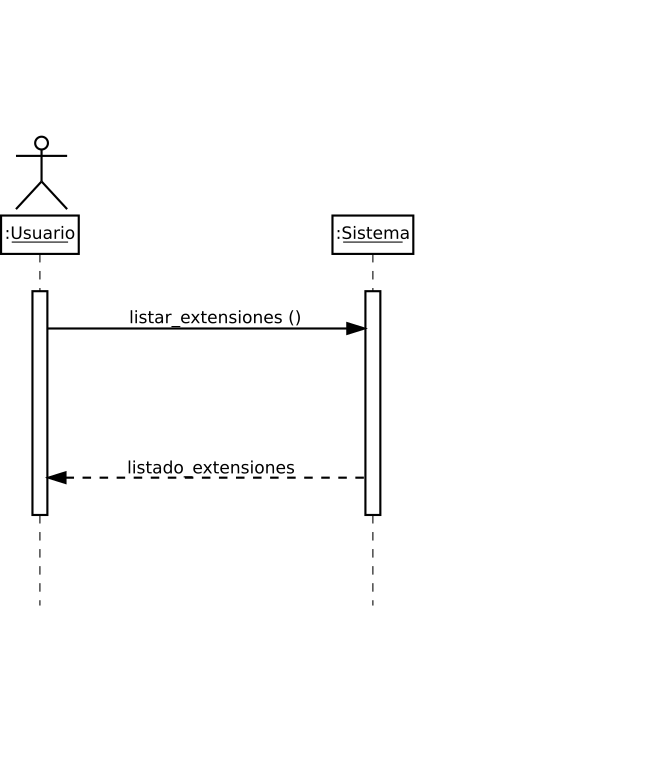
\includegraphics[scale=0.4]{listar_extensiones.png} \\
\end{center}

\section{Contratos de operaciones del sistema}
\begin{center}
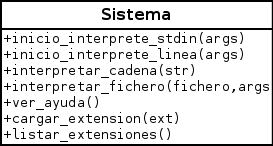
\includegraphics[scale=0.7]{operaciones_sistema.png} \\
\end{center}
\subsection{Operación inicio\_interprete\_stdin}
\FloatBarrier
\begin{framed}
	\begin{description}
		\item [Nombre:] inicio\_interprete\_stdin(args)
		\item [Responsabilidades:] Iniciar la interpretación de la entrada estándar.
		\item [Referencias Cruzadas: ] Caso de Uso: Interpretar entrada estándar
      \item [Precondiciones:] No tiene.
      \item [Postcondiciones:] \hfill
      \begin {itemize}
         \item Se creó una instancia ``i'' de ``interpreter'' (creación de objeto).
         \item Se inicializaron los atributos de ``i''.
         \item Se crearon las instancias ``$a_0...a_n$'' de ``arg'' por cada argumento en ``args'' (creación de objeto).
         \item Se asignó ``args$_i$'' a ``$a_i.value$'' ($a_i.value = $args$_i$) (modificación de atributos).
         \item Se asoció los ``arg'' ``$a_0...a_n$'' al objeto ``i'' de ``interpreter'' (creación de enlace).
         \item Se creó una instancia ``p'' de ``parser'' (creación de objeto).
         \item Se inicializaron los atributos de ``p''.
         \item Se creó una instancia ``s'' de ``scanner'' (creación de objeto).
         \item Se inicializaron los atributos de ``s''.
         \item Se asoció el ``scanner'' ``s'' al objeto ``p'' de ``parser'' (creación de enlace).
         \item Se asoció el ``parser'' ``p'' al objeto ``i'' de ``interpreter'' (creación de enlace).
         \item Se creó una instancia ``c'' de ``context'' (creación de objeto).
         \item Se inicializaron los atributos de ``c''.
         \item Se creó una instancia ``var'' de ``varSymbols'' (creación de objeto).
         \item Se inicializaron los atributos de ``var''.
         \item Se asoció el ``varSymbols'' ``var'' al objeto ``c'' de ``context'' (creación de enlace).
         \item Se creó una instancia ``func'' de ``funcSymbols'' (creación de objeto).
         \item Se inicializaron los atributos de ``func''.
         \item Se asoció el ``funcSymbols'' ``func'' al objeto ``c'' de ``context'' (creación de enlace).
         \item Se creó una instancia ``class'' de ``classSymbols'' (creación de objeto).
         \item Se inicializaron los atributos de ``class''.
         \item Se asoció el ``classSymbols'' ``class'' al objeto ``c'' de ``context'' (creación de enlace).
         \item Se asoció el ``context'' ``c'' al objeto ``i'' de ``interpreter'' (creación de enlace).
      \end{itemize}
	\end{description}
\end{framed}
\FloatBarrier

\subsection{Operación inicio\_interprete\_linea}
\FloatBarrier
\begin{framed}
	\begin{description}
		\item [Nombre:] inicio\_interprete\_linea(args)
		\item [Responsabilidades:] Iniciar la interpretación interactiva línea a línea.
		\item [Referencias Cruzadas: ] Caso de Uso: Interpretar línea
      \item [Precondiciones:] No tiene.
      \item [Postcondiciones:] \hfill
      \begin {itemize}
         \item Se creó una instancia ``i'' de ``interpreter'' (creación de objeto).
         \item Se inicializaron los atributos de ``i''.
         \item Se crearon las instancias ``$a_0...a_n$'' de ``arg'' por cada argumento en ``args'' (creación de objeto).
         \item Se asignó ``args$_i$'' a ``$a_i.value$'' ($a_i.value = $args$_i$) (modificación de atributos).
         \item Se asoció los ``arg'' ``$a_0...a_n$'' al objeto ``i'' de ``interpreter'' (creación de enlace).
         \item Se creó una instancia ``p'' de ``parser'' (creación de objeto).
         \item Se inicializaron los atributos de ``p''.
         \item Se creó una instancia ``s'' de ``scanner'' (creación de objeto).
         \item Se inicializaron los atributos de ``s''.
         \item Se asoció el ``scanner'' ``s'' al objeto ``p'' de ``parser'' (creación de enlace).
         \item Se asoció el ``parser'' ``p'' al objeto ``i'' de ``interpreter'' (creación de enlace).
         \item Se creó una instancia ``c'' de ``context'' (creación de objeto).
         \item Se inicializaron los atributos de ``c''.
         \item Se creó una instancia ``var'' de ``varSymbols'' (creación de objeto).
         \item Se inicializaron los atributos de ``var''.
         \item Se asoció el ``varSymbols'' ``var'' al objeto ``c'' de ``context'' (creación de enlace).
         \item Se creó una instancia ``func'' de ``funcSymbols'' (creación de objeto).
         \item Se inicializaron los atributos de ``func''.
         \item Se asoció el ``funcSymbols'' ``func'' al objeto ``c'' de ``context'' (creación de enlace).
         \item Se creó una instancia ``class'' de ``classSymbols'' (creación de objeto).
         \item Se inicializaron los atributos de ``class''.
         \item Se asoció el ``classSymbols'' ``class'' al objeto ``c'' de ``context'' (creación de enlace).
         \item Se asoció el ``context'' ``c'' al objeto ``i'' de ``interpreter'' (creación de enlace).
      \end{itemize}
	\end{description}
\end{framed}
\FloatBarrier

\subsection{Operación interpretar\_cadena}
\FloatBarrier
\begin{framed}
	\begin{description}
		\item [Nombre:] interpretar\_cadena(str)
		\item [Responsabilidades:] Interpreta el contenido fuente almacenado en la cadena ``str''
		\item [Referencias Cruzadas: ] \hfill
      \begin {itemize}
      \item Caso de Uso: Interpretar entrada estándar 
      \item Caso de Uso: Interpretar línea
      \end{itemize}
      \item [Precondiciones:] \hfill
      \begin {itemize}
      \item Se creó un ``interpreter'' ``i''.
      \item Se creó y asoció una instancia de ``parser'' y ``scanner'' a ``i''.
      \item Se creó y asoció una instancia de ``varSymblos'', ``funcSymbols'' y ``classSymbols'' a ``i''.
      \end{itemize}
      \item [Postcondiciones:] \hfill
      \begin {itemize}
         \item Se creó una instancia ``s'' de ``source'' (creación de objeto).
         \item Se asignó ``str'' a ``s.src'' (s.src = str) (modificación de atributos)
         \item Se asoció ``s'' al ``scanner'' componente del ``interpreter'' ``i'' (creación de enlace). 
         \item Se creó un conjunto ``$t_0...t_n$'' de ``token'' a partir del análisis léxico (creación de objeto).
         \item Se creó un conjunto ``$n_0...n_n$'' de ``runNode'' a partir del análisis sintáctico (creación de objetos).
         \item Se asoció ``$n_i\ \epsilon\ n_0...n_n$'' a ``$n_k\ \epsilon\ n_0...n_n$'' para construir el árbol sintáctico (creación de enlace).
         \item Se asoció  ``$n_r\ \epsilon\ n_0...n_n$'', raíz del árbol sintáctico, al ``interprter'' ``i'' (creación de enlace).
         %~ \item Se asignó cada valor ``$v_i$'', dado por la ejecución de ``$e_i\ \epsilon\ n_0...n_n$'' objeto de ``expNode'', a ``$e_i$.val'' ($e_i$.val = $v_i$)(modificación de atributos) 
         \item Se creó un conjunto ``$var_0...var_n$'' de ``refNode'' correspondientes a las variables definidas en el contenido fuente (creación de objetos).
         \item Se creó un conjunto ``$val_0...val_n$'' de ``runNode'' correspondientes a los valores asignados a las variables definidas en el contenido fuente (creación de objetos).
         \item Se asoció ``$val_i\ \epsilon\ val_0...val_n$'' a  ``$var_i\ \epsilon\ var_0...var_n$'' donde $val_i$ es el valor de la variable $var_i$ (creación de enlace). 
         \item Se asoció todo ``refNode'' ``$var_0...var_n$'' al componente ``varSymbols'' de ``i'' (creación de enlace). 
         \item Se creó un conjunto ``$func_0...func_n$'' de ``refNode'' correspondientes a las funciones con identificador definidas en el contenido fuente (creación de objetos).
         \item Se asoció ``$func_i\ \epsilon\ func_0...func_n$'' a  ``$n_i\ \epsilon\ n_0...n_n$'' donde $n_i$ es un ``funcNode'' correspondiente a la definición de la función $func_i$ (creación de enlaces).
         \item Se asoció todo ``refNode'' ``$func_0...func_n$'' al componente ``funcSymbols'' de ``i'' (creación de enlace). 
         \item Se creó un conjunto ``$class_0...class_n$'' de ``refNode'' correspondientes a las clases definidas en el contenido fuente (creación de objetos).
         \item Se asoció ``$class_i\ \epsilon\ class_0...class_n$'' a  ``$n_i\ \epsilon\ n_0...n_n$'' donde $n_i$ es un ``classNode'' correspondiente a la definición de la clase $class_i$ (creación de enlaces).
         \item Se asoció todo ``refNode'' ``$class_0...class_n$'' al componente ``classSymbols'' de ``i'' (creación de enlace). 
      \end{itemize}
	\end{description}
\end{framed}
\FloatBarrier

\subsection{Operación interpretar\_fichero}
\FloatBarrier
\begin{framed}
	\begin{description}
		\item [Nombre:] interpretar\_fichero(fichero, args)
		\item [Responsabilidades:] Interpreta el contenido fuente almacenado en ``fichero''
		\item [Referencias Cruzadas: ] Caso de Uso: Interpretar fichero
      \item [Precondiciones:] No tiene.
      \item [Postcondiciones:] \hfill
      \begin {itemize}
         \item Se creó una instancia ``i'' de ``interpreter'' (creación de objeto).
         \item Se inicializaron los atributos de ``i''.
         \item Se creó el conjunto ``$a_0...a_n$'' de ``arg'' según el número de argumentos en ``args'' (creación de objeto).
         \item Se asignó ``args$_i$'' a ``$a_i.value$'' ($a_i.value = $args$_i$) (modificación de atributos).
         \item Se asoció los ``arg'' ``$a_0...a_n$'' al objeto ``i'' de ``interpreter'' (creación de enlace).
         \item Se creó una instancia ``p'' de ``parser'' (creación de objeto).
         \item Se inicializaron los atributos de ``p''.
         \item Se creó una instancia ``s'' de ``scanner'' (creación de objeto).
         \item Se inicializaron los atributos de ``s''.
         \item Se asoció el ``scanner'' ``s'' al objeto ``p'' de ``parser'' (creación de enlace).
         \item Se asoció el ``parser'' ``p'' al objeto ``i'' de ``interpreter'' (creación de enlace).
         \item Se creó una instancia ``c'' de ``context'' (creación de objeto).
         \item Se inicializaron los atributos de ``c''.
         \item Se creó una instancia ``var'' de ``varSymbols'' (creación de objeto).
         \item Se inicializaron los atributos de ``var''.
         \item Se asoció el ``varSymbols'' ``var'' al objeto ``c'' de ``context'' (creación de enlace).
         \item Se creó una instancia ``func'' de ``funcSymbols'' (creación de objeto).
         \item Se inicializaron los atributos de ``func''.
         \item Se asoció el ``funcSymbols'' ``func'' al objeto ``c'' de ``context'' (creación de enlace).
         \item Se creó una instancia ``class'' de ``classSymbols'' (creación de objeto).
         \item Se inicializaron los atributos de ``class''.
         \item Se asoció el ``classSymbols'' ``class'' al objeto ``c'' de ``context'' (creación de enlace).
         \item Se asoció el ``context'' ``c'' al objeto ``i'' de ``interpreter'' (creación de enlace).
      
      
         \item Se creó una instancia ``src'' de ``source'' (creación de objeto).
         \item Se asignó el contenido de ``fichero'' a ``src.src'' (src.src = fichero) (modificación de atributos)
         \item Se asoció ``src'' al ``scanner'' ``s'' componente del ``interpreter'' ``i'' (creación de enlace). 
         \item Se creó un conjunto ``$t_0...t_n$'' de ``token'' a partir del análisis léxico (creación de objeto).
         \item Se creó un conjunto ``$n_0...n_n$'' de ``runNode'' a partir del análisis sintáctico (creación de objetos).
         \item Se asoció ``$n_i\ \epsilon\ n_0...n_n$'' a ``$n_k\ \epsilon\ n_0...n_n$'' para construir el árbol sintáctico (creación de enlace).
         \item Se asoció  ``$n_r\ \epsilon\ n_0...n_n$'', raíz del árbol sintáctico, al ``interprter'' ``i'' (creación de enlace).
         %~ \item Se asignó cada valor ``$v_i$'', dado por la ejecución de ``$e_i\ \epsilon\ n_0...n_n$'' objeto de ``expNode'', a ``$e_i$.val'' ($e_i$.val = $v_i$)(modificación de atributos) 
         \item Se creó un conjunto ``$var_0...var_n$'' de ``refNode'' correspondientes a las variables definidas en el contenido fuente (creación de objetos).
         \item Se creó un conjunto ``$val_0...val_n$'' de ``runNode'' correspondientes a los valores asignados a las variables definidas en el contenido fuente (creación de objetos).
         \item Se asoció ``$val_i\ \epsilon\ val_0...val_n$'' a  ``$var_i\ \epsilon\ var_0...var_n$'' donde $val_i$ es el valor de la variable $var_i$ (creación de enlace). 
         \item Se asoció todo ``refNode'' ``$var_0...var_n$'' al componente ``varSymbols'' de ``i'' (creación de enlace). 
         \item Se creó un conjunto ``$func_0...func_n$'' de ``refNode'' correspondientes a las funciones con identificador definidas en el contenido fuente (creación de objetos).
         \item Se asoció ``$func_i\ \epsilon\ func_0...func_n$'' a  ``$n_i\ \epsilon\ n_0...n_n$'' donde $n_i$ es un ``funcNode'' correspondiente a la definición de la función $func_i$ (creación de enlaces).
         \item Se asoció todo ``refNode'' ``$func_0...func_n$'' al componente ``funcSymbols'' de ``i'' (creación de enlace). 
         \item Se creó un conjunto ``$class_0...class_n$'' de ``refNode'' correspondientes a las clases definidas en el contenido fuente (creación de objetos).
         \item Se asoció ``$class_i\ \epsilon\ class_0...class_n$'' a  ``$n_i\ \epsilon\ n_0...n_n$'' donde $n_i$ es un ``classNode'' correspondiente a la definición de la clase $class_i$ (creación de enlaces).
         \item Se asoció todo ``refNode'' ``$class_0...class_n$'' al componente ``classSymbols'' de ``i'' (creación de enlace). 
      \end{itemize}
	\end{description}
\end{framed}
\FloatBarrier
% ----------------------------------------------------------------------
